Wie können Computer so viele unterschiedliche Dinge mit nur Nullen und Einser darstellen? Auf dem Bildschirm sehen wir Texte, Bilder, Videos, die wir noch dazu verändern können.

Vorletzte Woche haben wir gesehen, wie Computer ganze Zahlen speichern und manipulieren. Sie stellen die Zahlen in Basis 2 dar und speichern eine feste Anzahl Bits.

\begin{aufgabe}
Schreibe folgende Zahlen in der 32-Bit Zweierkomplement Darstellung:
\begin{enumerate}[(a)]
\item \(5\)
\item \(-1\)
\item \(25\)
\item \(-25\)
\end{enumerate}
\end{aufgabe}

Letzte Woche haben wir angefangen, uns mit der Darstellung der reellen Zahlen zu beschäftigen, mit den \textbf{Fliesskommazahlen}. Heute machen wir damit weiter.

Die Fliesskommazahlen, wie wir gesehen haben, sind im Grunde genommen nichts anderes, als die \textbf{Exponentialschreibweise}, die wir schon aus Chemie und Physik kennen: Die \textbf{Mantisse} wird mit der Basis hoch einem \textbf{Exponenten} multipliziert.

Zum Beispiel, die Avogadro-Konstante schreiben die Chemiker als \(6.02214076 \cdot 10^{23}\), anstatt alle 24 Stellen anzugeben. In dieser Schreibweise lassen sich Zahlen der unterschiedlichsten Grössenordnungen kompakt und übersichtlich darstellen:
\begin{itemize}
\item Masse von einem Proton: \(1.673 \cdot 10^{-27}\) Kilogramm
\item Grösse eines Coronavirus: \(1,4 \cdot 10^{-7}\) Meter
\item Lichtgeschwindigkeit: \(2.998 \cdot 10^{8}\) Meter pro Sekunde
\item Durchmesser von der Andromedagalaxie: \(1.32 \cdot 10^{21}\) Meter
\end{itemize}

Im Unterschied zu Menschen, arbeitet der Computer meistens in der Basis \(2\) statt \(10\) und \textbf{schränkt} die Anzahl der möglichen signifikanten Stellen und Exponenten \textbf{ein}.

Um diese Einschränkungen sichtbar und anfassbar zu machen, hatten wir das \textbf{''Kasten-Seil''-Modell} eingeführt.

\begin{figure}[H]
\centering
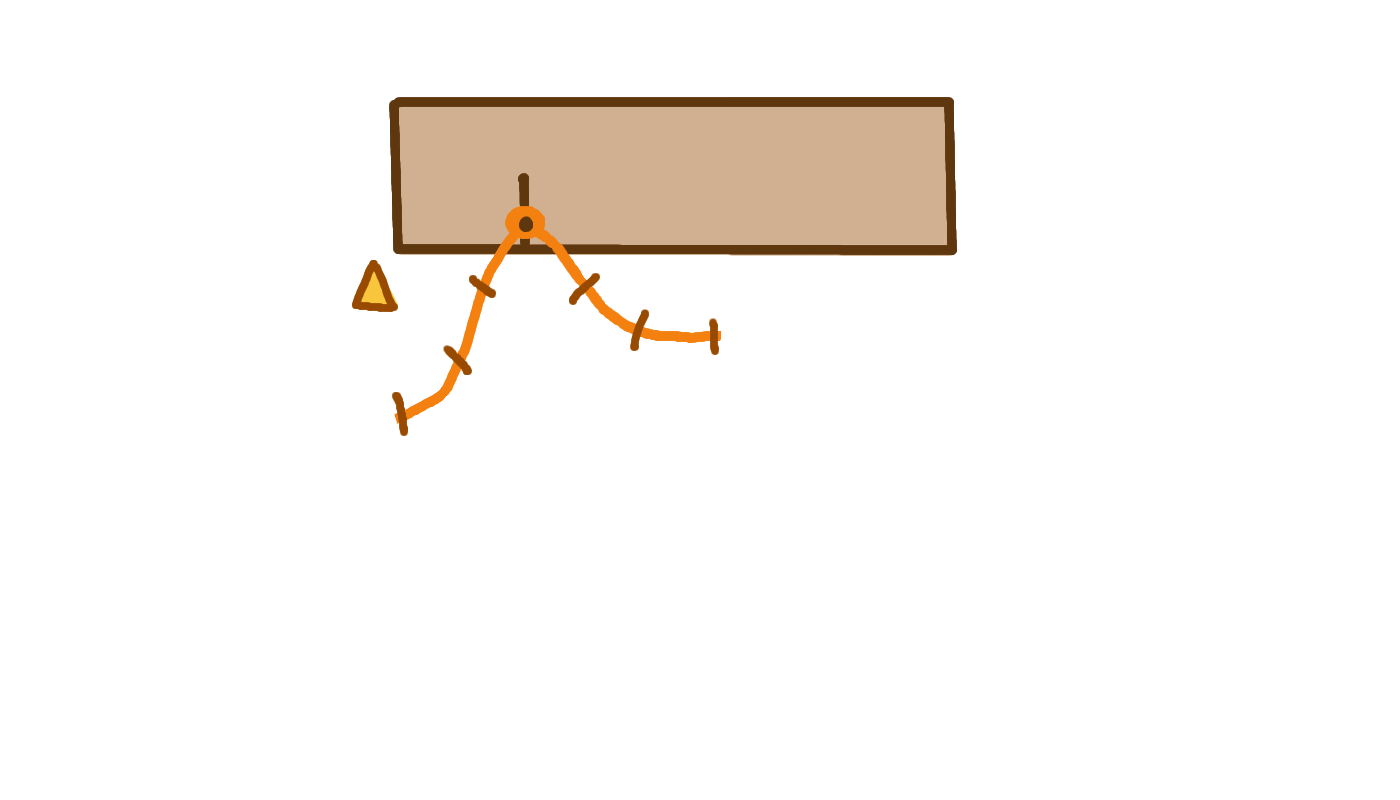
\includegraphics[width=0.75\linewidth]{Pictures/KastenOhneZahlen.png} 
\end{figure}

Das Modell besteht aus einem \textbf{Kasten}, in welchem wir eine fixe Anzahl Ziffern speichern können, und einem \textbf{Seil}, welches die Position vom Kasten bezüglich dem Komma speichert. Die Mitte vom Seil ist genau nach der ersten Stelle im Kasten befestigt und zwei Enden hängen lose: Das \textbf{negative Ende}  und das \textbf{positive Ende}. Auf dem Seil wird \textbf{markiert}, wo sich das Komma befindet.

Was machen wir, wenn wir folgende reelle Zahlen, binär in einer Fixkommadarstellung dargestellt, im ''Kasten-und-Seil''-Modell umschreiben wollen?

\begin{figure}[H]
\centering
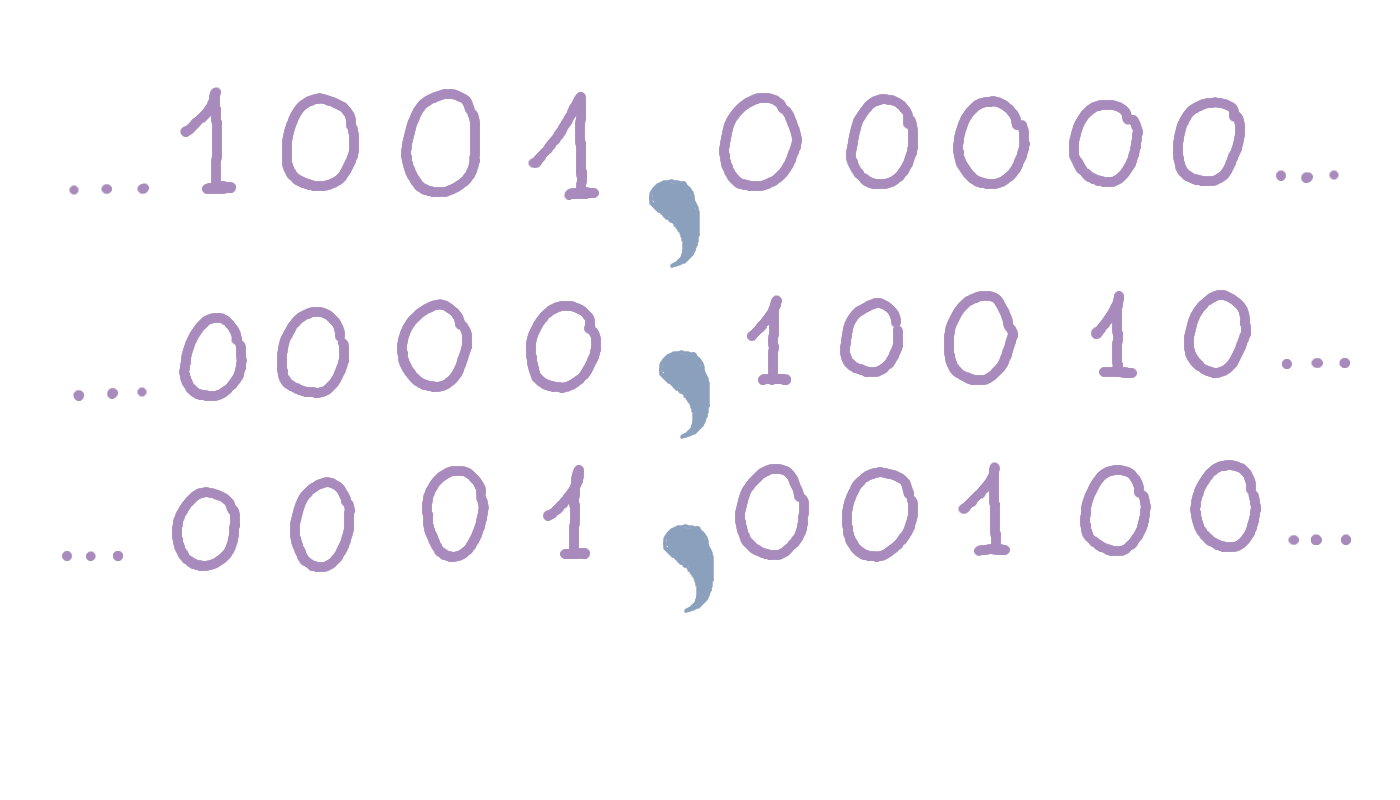
\includegraphics[width=0.65\linewidth]{Pictures/Zahlengerade.png} 
\end{figure}

Erstens, müssen wir bestimmen, wo wir den Kasten hinstellen, d.h. welche Ziffern gespeichert werden. Alle Ziffern, die sich ausserhalb vom Kasten befinden, gehen verloren. Es macht Sinn, die Ziffern mit dem grössten Wert zu nehmen, also mit der linkesten Eins anzufangen. Die Bits im Kasten sind die \textbf{Mantisse}.

\begin{figure}[H]
\centering
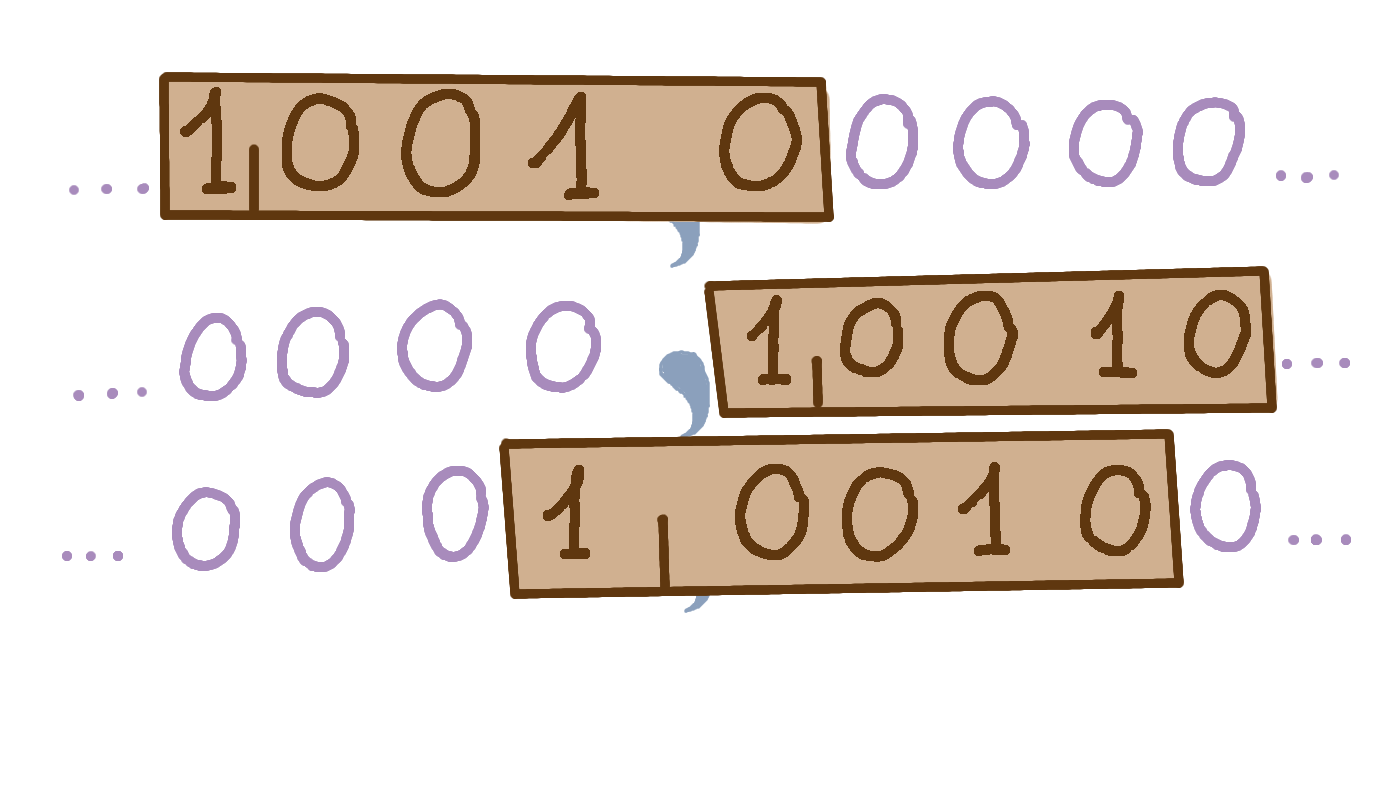
\includegraphics[width=0.65\linewidth]{Pictures/Kasten.png} 
\end{figure}

Nun haben wir 3 Kasten mit genau dem gleichen Inhalt: \texttt{10010}. Um die ursprünglichen Zahlen rekonstruieren zu können, müssen wir uns auch die Position des Kastens bezüglich dem Komma merken. Das machen wir im zweiten Schritt mit dem Seil. Die Mitte vom Seil wird gleich nach der linkesten Ziffer im Kasten befestigt, und die Position vom Komma wird am Seil markiert. Die Markierung auf dem Seil modelliert den \textbf{Exponenten}.

\begin{figure}[H]
\centering
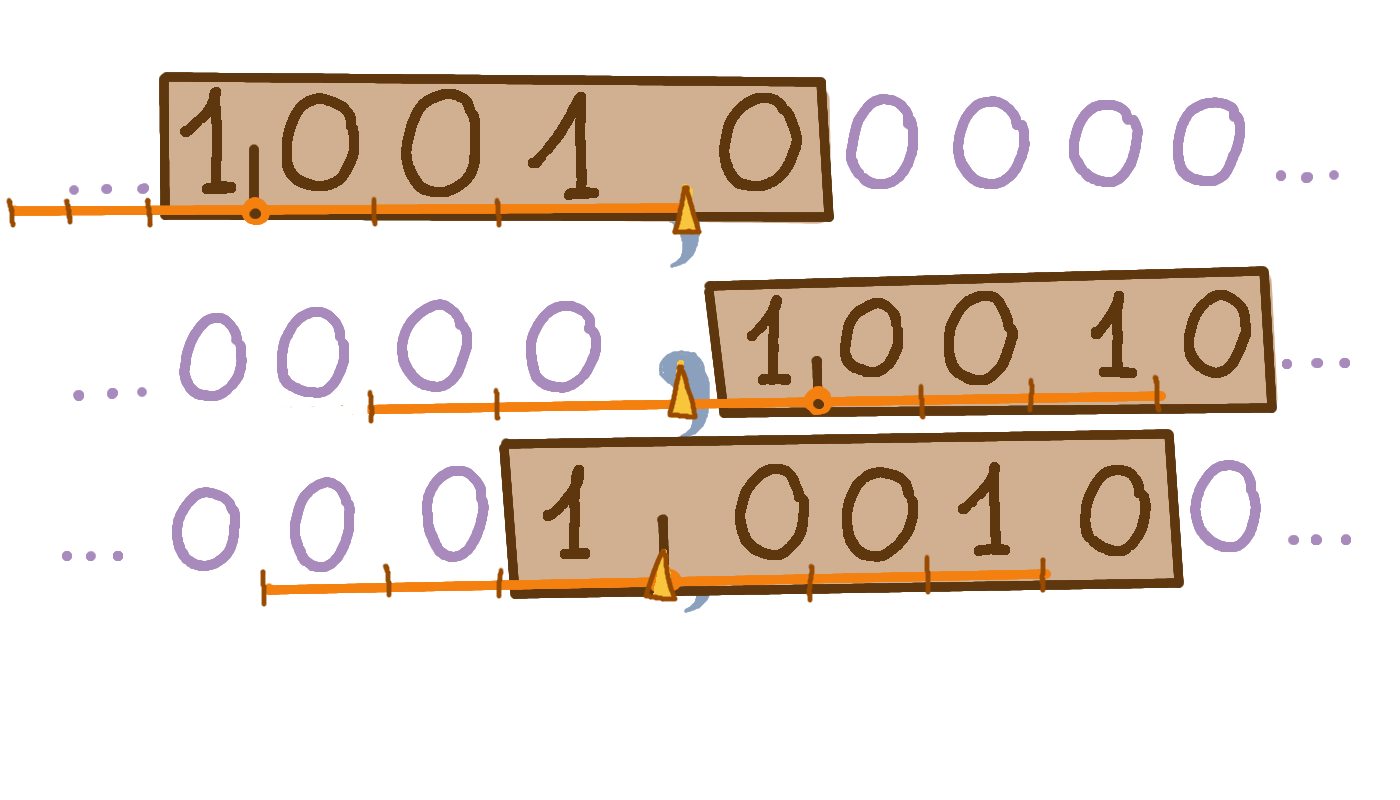
\includegraphics[width=0.65\linewidth]{Pictures/KastenMitSeil.png} 
\end{figure}

Jetzt haben wir alle Informationen gespeichert, die wir brauchen, um die ursprünglichen Zahlen wiederherzustellen. Damit diese Darstellung eindeutig ist, verlangen wir, dass das erste Bit der Mantisse eine Eins ist.

Folgende Elemente charakterisieren ein Fliesskommazahlensystem: Die Grösse vom Kasten, d.h. die \textbf{Mantissenlänge}, und die Länge vom Seil, d.h. der \textbf{Exponentenbereich}. Die Bits im Kasten und die Markierung am Seil stellen eine Zahl dar.

Der Computer hat intern keine Kasten und keine Seile. Er arbeitet mit Bitmuster. Jede Zahl hat eine fixe Anzahl Bits, typischerweise 32 (float) oder 64 (double), und diese Bits werden in \(3\) Bereiche aufgeteilt:
\begin{itemize}
\item Vorzeichen (grün auf dem Bild),
\item Exponent (Orange auf dem Bild),
\item Mantisse (braun auf dem Bild). 
\end{itemize}
Im Vorzeichenteil wird das \textbf{Vorzeichen} kodiert: \texttt{0} für positive Zahlen und \texttt{1} für negative.

Im Exponententeil wird die Markierung am Seil kodiert. Damit positive und negative Exponente in der fixen Anzahl Bits kodiert werden können, ein  \textbf{Biaswert} wird zum Exponenten addiert, so dass die \(0\) mit \texttt{1000...0} kodiert wird.

Im Mantissenteil werden die Bits aus dem Kasten gespeichert. Da das erste Bit immer eine Eins ist, wird es im Computer nicht gespeichert (implizites oder verstecktes Bit). Hier wird deshalb die führende Eins immer in Klammern angeführt.
\begin{figure}[H]
\centering
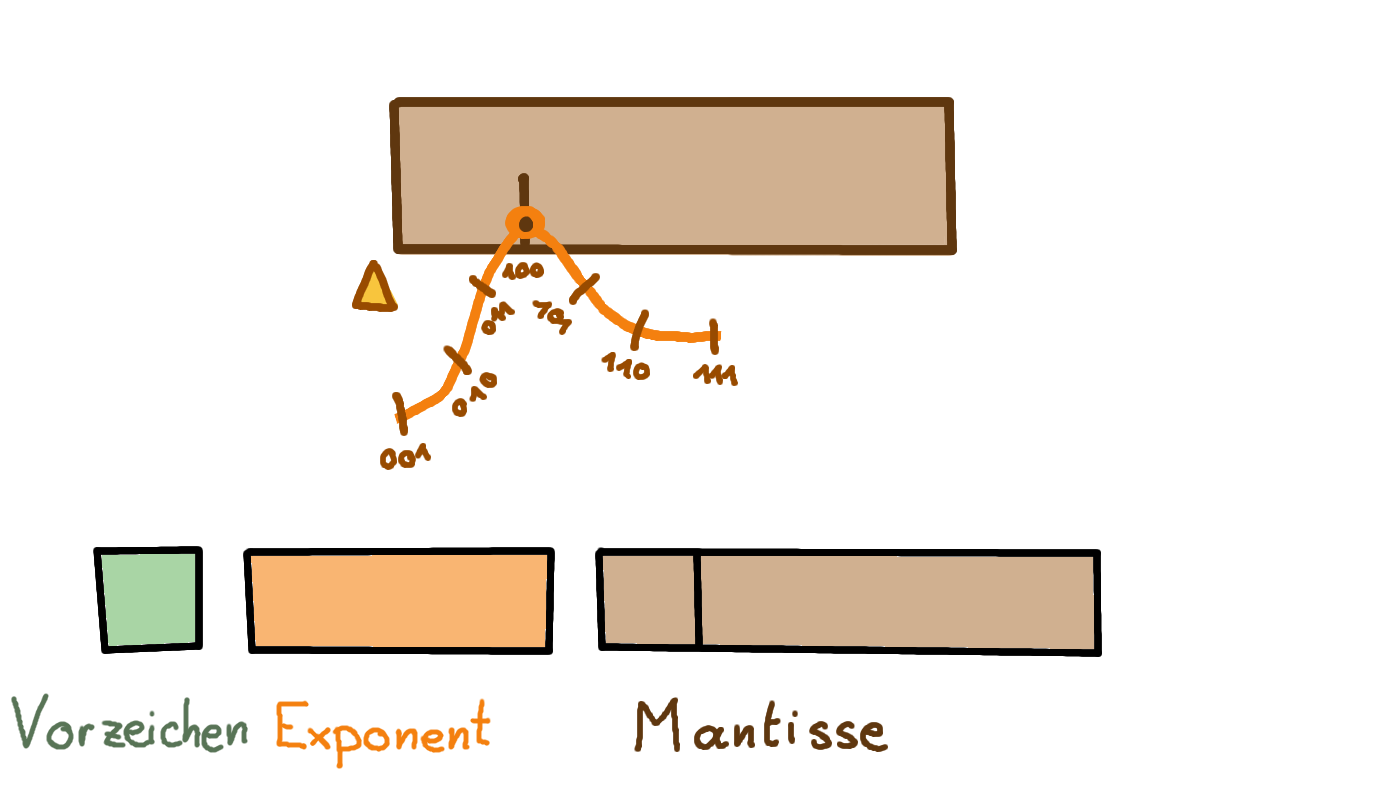
\includegraphics[width=0.75\linewidth]{Pictures/KastenMitSpeicher.png} 
\end{figure}

\begin{beispiel}
Wir werden zusammen die Zahl \(6.5\) im Fliesskommazahlensystem mit Mantissenlänge \(5\) und Exponenten von \(-3\) bis \(3\) darstellen.

Die reelle Zahl in Basis 2 in einer Fixkommadarstellung ist \(110.1\).

Der Kasten hat 5 Plätze. Alle signifikanten Stellen haben dort Platz. Dann verbinden wir das Seil mit dem Komma und setzen eine Markierung. Das lässt sich direkt ins Bitmuster übersetzen: Das Vorzeichen ist positiv, die Kodierung vom Exponenten lässt sich am Seil ablesen, die Mantisse speichert man direkt.
\begin{figure}[H]
\centering
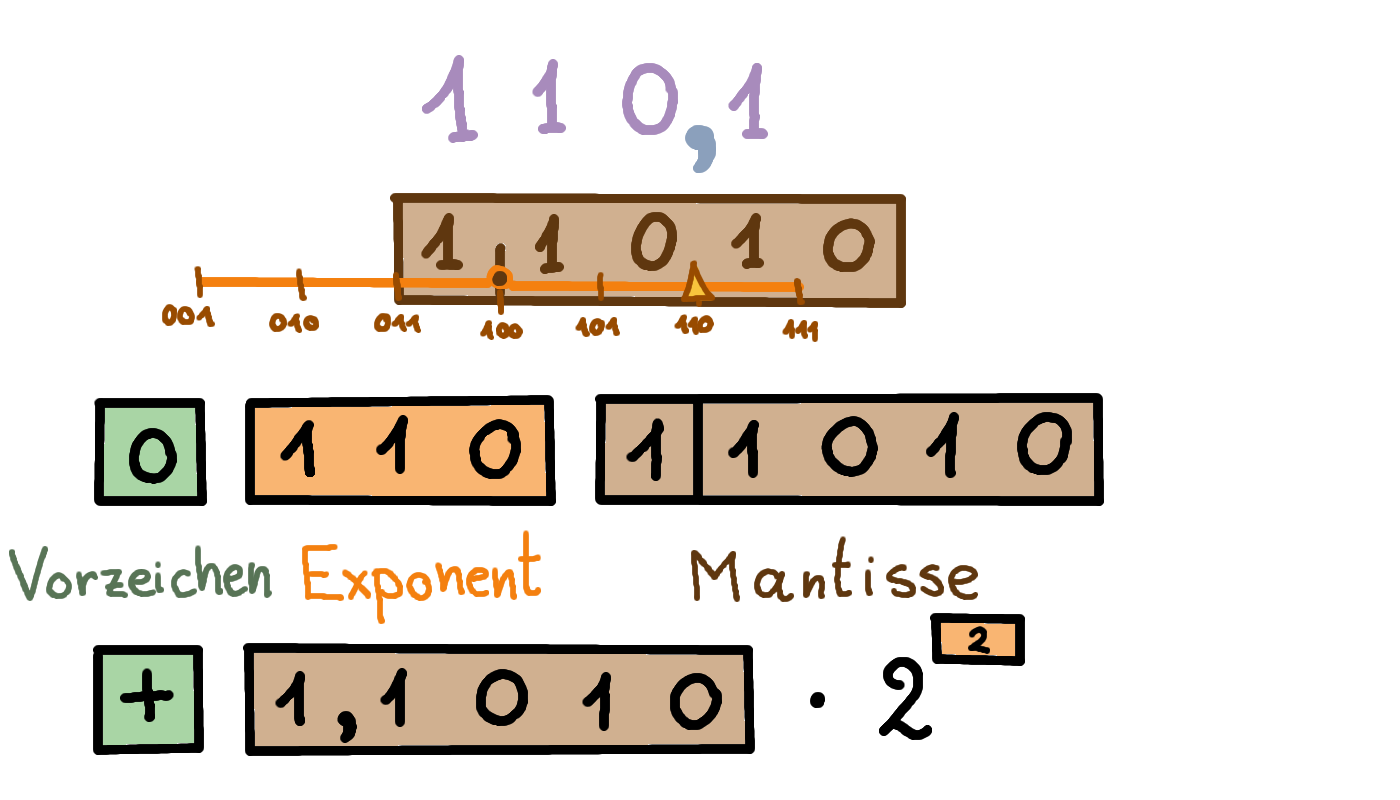
\includegraphics[width=0.75\linewidth]{Pictures/ZahlenDarstellen6-5.png} 
\end{figure}

\end{beispiel}

\begin{aufgabe}\label{einleitung-vom-kasten-nach-zahl}
Welche Zahl ist unten dargestellt? Vervollständige das Bitmuster und die Exponentialschreibweise und schreibe den Dezimalwert auf.

\begin{figure}[H]
\centering
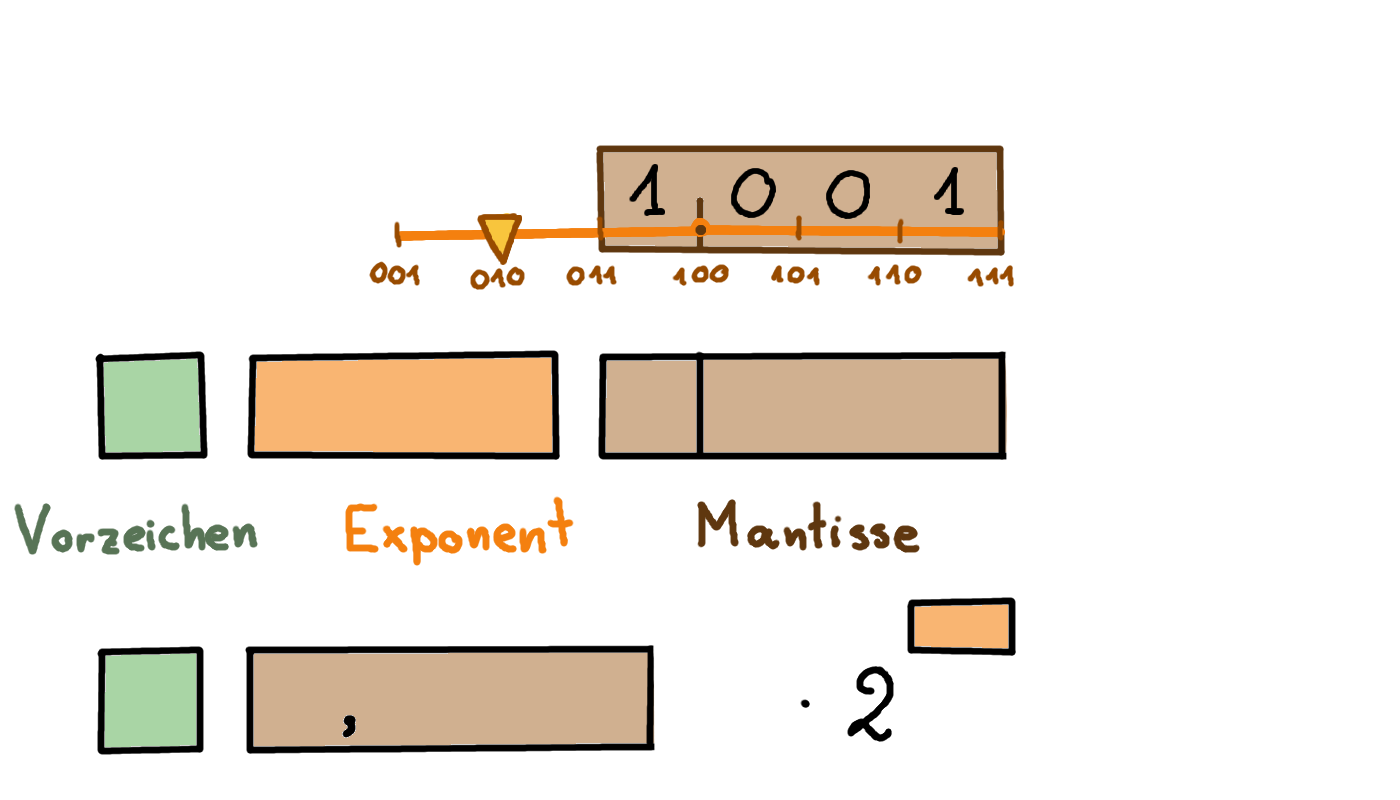
\includegraphics[width=0.8\linewidth]{Pictures/Einleitung_from_Kasten.png} 
\end{figure}
\end{aufgabe}

\begin{beispiel}
Nicht alle Zahlen lassen sich im Fliesskommazahlensystem genau darstellen. Manche müssen gerundet werden.
Zum Beispiel, die Zahl \(10.75\) sieht in Binär in einer Fixkommadarstellung so aus: \(1010.11\). Sie hat \(6\) signifikante Stellen, aber nur \(5\) haben in der Mantisse Platz. Die letzte Eins kann nicht gespeichert werden und geht verloren.
\begin{figure}[H]
\centering
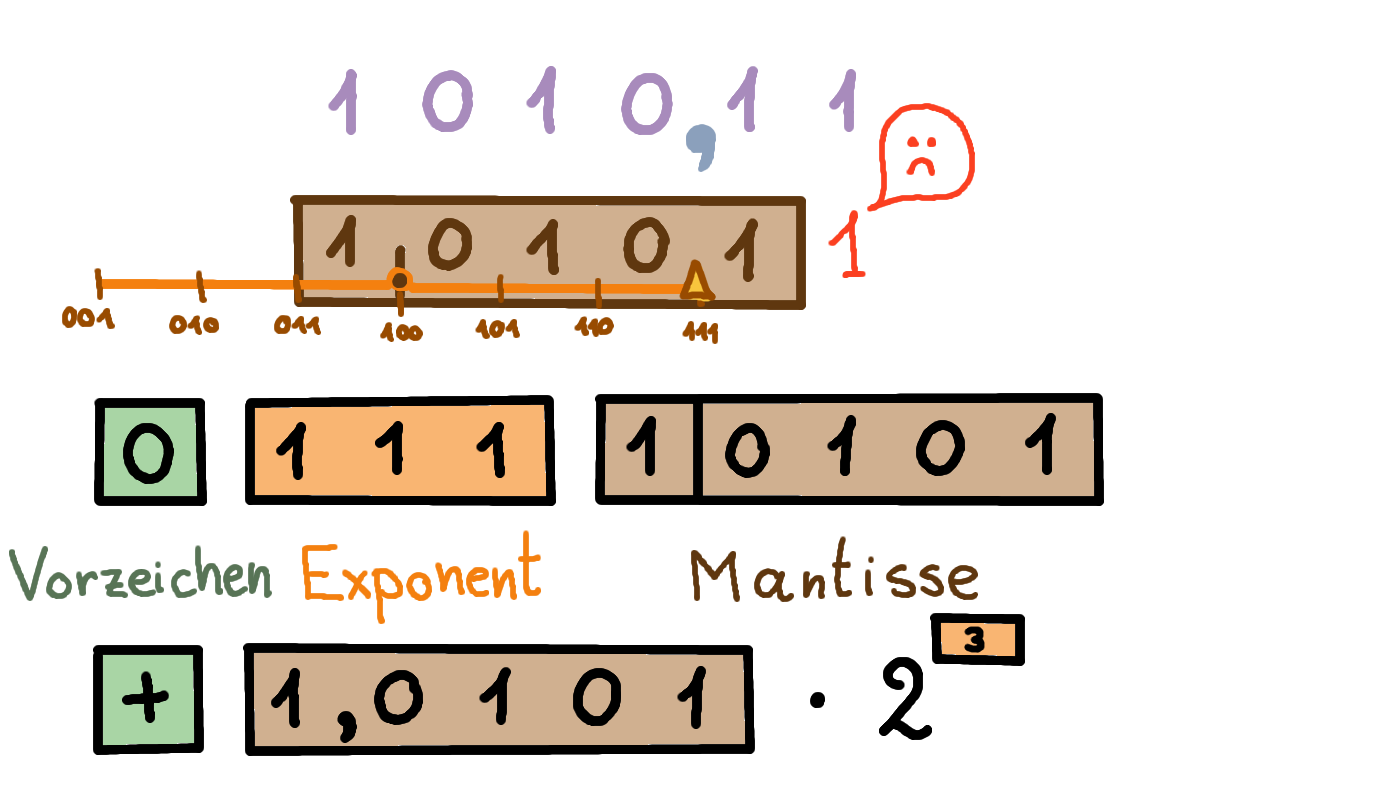
\includegraphics[width=0.75\linewidth]{Pictures/ZahlenDarstellen10-75.png} 
\end{figure}

\end{beispiel}